\documentclass[12pt]{article}


\usepackage{tikz}
\usetikzlibrary{calc}


\begin{document}
{
		\def\labels{1}
\def\check#1{
        \ifdefined \labelss
            #1
        \fi
    } 


        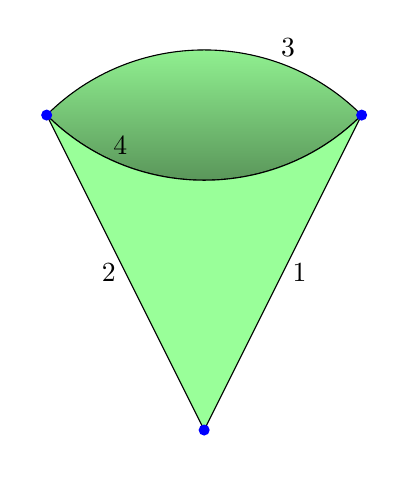
\begin{tikzpicture}[edge/.style={fill=yellow}, faceColor/.style={green!40!white}, face/.style={fill=faceColor/.style, draw=black}]
			\def\scale{2}        
        
               \coordinate [label={[gray]below:\ifdefined \labels \check{1} \fi}] (A) at (0,0);

	        \coordinate [label=right:\ifdefined \labels \textcolor{blue}{2} \fi] (B) at (1*\scale,2*\scale);
	        \coordinate [label=left:\ifdefined \labels \textcolor{blue}{3} \fi] (C) at (-1*\scale,2*\scale);
			
			\def\col{green!40!white}
			
	        \filldraw[bottom color=\col!53!black, top color=green!40!white] (B) to[bend right=45] node[above, near start]{3} (C) to[bend right=45] (B);
			%\draw[dashed] (B) to[bend left=45] (C);	        
	        \filldraw[fill=green!40!white] (A) -- node[right]{1} (B) to[bend left=45]node[above, near end]{4} (C) -- node[left]{2} cycle;
	        
	        \ifdefined \labels
	        	% Draw face labels
	        	\node at ($1/2*(A)+1/4*(B)+1/4*(C)$) {I};
	        	\node at ($1/2*(B)+1/2*(C)$) {II};	        	
	        \fi
	        
	        \foreach \x in {A,B,C}
	        	\fill[blue] (\x) circle (2pt);
	    \end{tikzpicture}
 
   }         
            
\end{document}